\documentclass[twocolumn]{article}
\usepackage[polish]{babel}
\usepackage[backend=biber,style=numeric]{biblatex}
\usepackage{graphicx}
\usepackage[hidelinks]{hyperref}
\usepackage{listings}
\usepackage{amsmath}
\usepackage{tikz}
\usepackage{pgfplots}

\lstset{
    captionpos=b,
    frame=single,
    language=Python,
    basicstyle=\footnotesize\ttfamily,
    float,
    floatplacement=H,
}

\bibliography{bibliography}

\title{Wybór języków programowania w modelu PGAS do porównania}
\author{Kamil Jarosz \and Wiktor Sus \and Michał Śledź}

\begin{document}
\maketitle

\section{PGAS}

Model PGAS jest modelem łączącym pewne cechy modelu \textit{Shared Memory} (SM)
oraz modelu \textit{Message Passing} (MP).
W modelu tym mamy jedną globalną pamięć widoczną dla równoległego programu jako całość, jednak pod spodem
pamięć ta może być rozproszona.
Z tego powodu czas dostępu do pamięci jest niejednolity tj.\ dostęp do pamięci,
która nie jest fizycznie na maszynie uruchamiającej program będzie dłuższy.

Rysunek~\ref{fig:mem_models} przedstawia wspomniane 3 modele pamięci.
Okręgami zostały zaznaczone procesy, natomiast prostokątami pamięć.
W modelu MP dostęp do pamięci danego procesu następuje tylko przez ten proces,
podczas gdy w modelu SM każdy proces ma dostęp
do całej przestrzeni adresowej w sposób bezpośredni.
Model PGAS łączy cechy obu modeli powodując, że każdy proces ma oddzielną pamięć oraz
może bezpośrednio odwoływać się do pamięci innego procesu.
Pamięci procesów nie tworzą jednej fizycznej pamięci.

\begin{figure}[h]
    \centering
    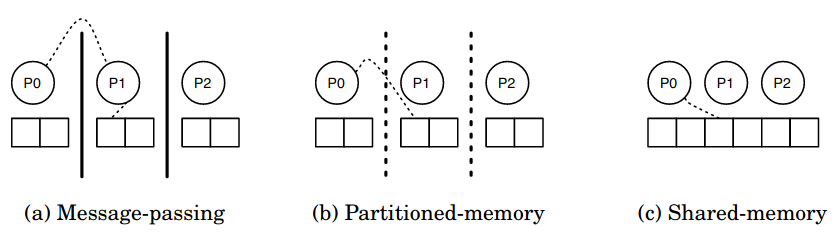
\includegraphics[width=\columnwidth]{mem_models.png}
    \caption{Modele pamięci~\cite{pgas_paper}}
    \label{fig:mem_models}
\end{figure}

Model PGAS cieszył się dużym wsparciem.
Powstało wiele rozszerzeń do języków, a nawet samodzielnych języków,
które umożliwiały z nim integrację.

\section{Języki modelu PGAS}

\subsection{CAF}
\label{ssec:caf}

Coarray Fortran (CAF)~\cite{coarray_fortran} jest rozszerzeniem Fortrana 95/2003,
który wprowadza elementy programowania równoległego.
Pozwala definiować tablice rozpięte na wszystkie \textit{obrazy}.
Obrazem nazywana jest kazda rozdystrybuowana kopia programu.
Ponadto pozwala na takie rzeczy jak synchronizacja wszystkich obrazów
lub dostęp do ich identyfikatorów.
Nie jest on wspierany od ponad 10 lat.

\subsection{Titanium}

\begin{figure}
    \centering
    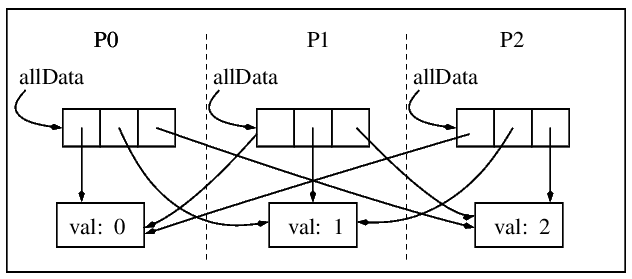
\includegraphics[width=\columnwidth]{titanium_memory.png}
    \caption{Przykładowy schemat pamięci dla tablicy rozpiętej na trzech procesach~\cite{titanium_docs}}
    \label{fig:titanium_memory}
\end{figure}

Titanium~\cite{titanium} jest dialektem Javy, który
pozwala na wprowadzenie abstrakcji nad równoległością.
Uniemożliwia on bezpośrednie używanie wątków, ale za to udostępnia
takie mechanizmy jak:
\begin{itemize}
    \item bariery,
    \item zmienne współdzielone między procesami,
    \item rozgłaszanie zmiennych pomiędzy procesy,
    \item tablice rozpięte na wszystkich procesach,
\end{itemize}
oraz wiele innych.
Ostatnia jego wersja była kompatybilna z Javą 1.4.
Przykładowy schemat tablicy w Titanium jest
przedstawiony na rysunku~\ref{fig:titanium_memory}.

\subsection{UPC}

Unified Parallel C (UPC)~\cite{upc} jest rozszerzeniem do języka C,
który wprowadza elementy programowania równoległego.
Podstawowe cechy:
\begin{itemize}
    \item Model wykonywania SPMD --- Single Program Multiple Data.
    \item Stała liczba tzw.\ \textit{places} nazywanych tutaj wątkami.
    Może być wybrana statycznie --- podczas kompilacji lub dynamicznie --- podczas wykonania.
    \item Domyślnie deklarowane zmienne zmienna są prywatne.
    Jeżeli jakaś dana ma być wspóldzielona oznacza się ją słowem kluczowym \textit{shared}.
    \item Dostęp do danych prywatnych i współdzielonych następuje w ten sam sposób.
    \item Posiada dodatkową instrukcję sterującą \texttt{upc\_forall}, za pomocą której
    możemy określić która iteracja pętli ma być wykonana przez który wątek.
\end{itemize}

Ostatnia wersja języka pochodzi z roku 2013~\cite{upc},
natomiast istnieje wiele implementacji, które są nadal
rozwijane~\cite{berkleyupc, upc_clang}.

\subsection{UPC++}

UPC++~\cite{upcxx} jest biblioteką do języka C++, która
pozwala na użycie modelu PGAS.
Podstawowe cechy:
\begin{itemize}
    \item aktywnie rozwijany --- ostatnia wersja wydana 12 marca 2020r.,
    \item jest odpowiednikiem UPC napisanym dla języka C++,
    \item ma dużo ciekawych funkcjonalności jak np.\ RPC (Remote Procedure Calls)
    czy początkowe wsparcie dla Nvidia CUDA~\cite{upcpp}.
\end{itemize}

\subsection{Chapel}

W przeciwieństwie do poprzednich narzędzi,
Chapel jest językiem programowania zaprojektowanym na potrzeby obliczeń równlogełych na wielką skalę.
Jego głównym założeniem implementacyjnym jest przenośność, która pozwala na uruchamianie go
na domowych komputerach i laptopach, klastrach oraz chmurach obliczeniowych oprócz wspieranych domyślnie
wydajnych superkomputerów, dla których został zaprojektowany.
Podstawowe cechy:
\begin{itemize}
    \item tzw. \textit{execution model} APGAS --- Asynchronous PGAS,
    \item zawiera mechanizmy \textit{implicit paralellism}, na przykład pętla \textit{forall},
    \item możliwe deklarowanie zmiennych w konkretnym \textit{place},
    \item wprowadza zarówno \textit{implicit} jak i \textit{explicit} \textit{remote data access},
    \item aktywnie rozwijany jako projekt open-source,
    \item posiada bogatą w przykłady dokumentację i materiały pozwalające na szybką
    i prostą naukę.
\end{itemize}

\subsection{XCalableMP}

Rozszerzenie dla języka C i Fortran przypominające OpenMP.
Wzorowane na HPF (High Performance Fortran~\cite{pgas_paper}) oraz
CAF (Co-array Fortran, opisany w sekcji~\ref{ssec:caf}).
Jest to zbiór dyrektyw kompilatora.
Podstawowe cechy:
\begin{itemize}
    \item Model wykonywania SPMD --- Single Program Multiple Data
    \item \textit{Explicit data distribution} oraz \textit{explicit remote data access}
    \item ostatnia specyfikacja pochodzi z listopada 2018 roku~\cite{xmphome}
\end{itemize}

\section{Wstępna analiza wybranych narzędzi}

\subsection{UPC++}

Instalacja biblioteki UPC++ nie jest trywialna.
Należy skompilować ją ze źródeł, gdyż nie jest ona udostępniania w postaci
binarnej na żadną dystrybucję.
Nie instaluje się ona również w standardowy sposób --- wykorzystuje ona własne
ścieżki w systemie (np. \texttt{/usr/local/upcxx}).
Przez to nie integruje się ona w łatwy sposób ze standardowymi narzędziami,
oraz wymaga ona własnego wrappera na kompilator (o nazwie \texttt{upcxx}).

Aby uruchomić skompilowany kod, należy użyć narzędzia \texttt{upcxx-run},
które jako jeden z argumentów przyjmuje liczbę procesów, na których uruchomić kod.
Jest to mały skrypt Pythonowy, pomagający w równoległym uruchomieniu programu.

Samo pisanie kodu za pomocą UPC++ jest analogiczne do używania
zwykłej biblioteki C++.
Kod korzystający z funkcji UPC++ musi być otoczony wywołaniami funkcji
\texttt{upcxx::init()} oraz \texttt{upcxx::finalize()}.
Większość funkcji dostępna jest z kontekstu statycznego z
przestrzeni nazw \texttt{upcxx}.
Przykładowe funkcje:
\begin{description}
\item[\texttt{upcxx::rank\_n()}] funkcja zwracająca liczbę wszystkich procesów,
\item[\texttt{upcxx::rank\_me()}] funkcja zwracająca identyfikator procesu,
\item[\texttt{upcxx::barrier()}] funkcja synchronizująca wszystkie procesy do tego miejsca
(analogiczna do standardowych funkcji OpenCL lub CUDA).
\end{description}

UPC++ również udostępnia parę typów, które ułatwiają zarządzanie pamięcią.
Na przykład \texttt{upcxx::global\_ptr} definiuje wskaźnik na obiekt, który
przechowywany jest w pamięci współdzielonej danego procesu.
Proces, który zdefiniował dany wskaźnik globalny może go
przekonwertować do wskaźnika standardowego C++ i używać
bez wykonywania specjalnych funkcji.
Jeśli natomiast dany proces nie jest właścicielem pamięci,
Jeśli stworzył on ten wskaźnik to jest go w stanie
musi użyć funkcji \texttt{upcxx::rget} i \texttt{upcxx::rput} aby
odpowiednio odczytać i zapisać wartość obiektu.

Aby rozdystrybuować wskaźnik na inne procesy, należy
użyć typu \texttt{upcxx::dist\_object}, który pozwala pobrać
wskaźnik z dowolnego innego procesu.
Służy do tego metoda \texttt{fetch}.
Przykład kodu dostępny jest na listingu~\ref{lst:upcxx-example}.

\begin{lstlisting}[
    caption=Korzystanie z pamięci współdzielonej w UPC++,
    label={lst:upcxx-example}]
upcxx::global_ptr<int> variable_ptr =
    upcxx::new_<int>(42);
upcxx::dist_object<upcxx::global_ptr<int>>
    variable(variable_ptr);

// variable from process 0
upcxx::global_ptr<int> variable_0 =
    variable.fetch(0).wait();
// variable from process 1
upcxx::global_ptr<int> variable_1 =
    variable.fetch(1).wait();
\end{lstlisting}

Obiekty typu \texttt{upcxx::future} są wszechobecne
i reprezentują klasyczne future'y.
Zwracane są one w przypadku uruchamiania funkcji
i metod, które mogą nie być natychmiastowe,
na przykład pobieranie wartości zmiennej z innego
procesu lub wykonanie RPC.

Przykład zastosowania tego drugiego obrazuje listing~\ref{lst:upcxx-rpc-example}.
\begin{lstlisting}[
    caption=Zastosowanie RPC w UPC++,
    label={lst:upcxx-rpc-example}]
upcxx::future<int> fut_result =
    upcxx::rpc(n, square, 2, 3);
int result = fut_result.wait();
\end{lstlisting}
Funkcja \texttt{square} jest funkcją wyliczającą pole prostokąta.
Do funkcji \texttt{upcxx::rpc()} przekazujemy nr procesu, na którym
ma zostać wykonana funkcja, nazwę samej funkcji, oraz jej argumenty.

W przypadku kiedy wykonujemy wiele obliczeń asynchronicznie,
zarządanie wszystkimi future'ami może być dosyć ciężkie, dlatego
UPC++ umożliwia grupowanie future'ów celem ich łatwiejszego zarządzania.
\begin{lstlisting}[
    caption=Grupowanie future w UPC++,
    label={lst:upcxx-conjoining-future}]
upcxx::future<int> fut_all =
    upcxx::make_future();
for (long i = 0; i < N; i++) {
    upcxx::future<int> fut =
        upcxx::rpc(n, square, 2, 3);
    fut_all =
        upcxx::when_all(fut_all, fut);
    if (i % 10 == 0) upcxx::progress();
}
fut_all.wait();
\end{lstlisting}
Listing~\ref{lst:upcxx-conjoining-future} przedstawia przykładowe wykorzystanie
wspomnianego mechanizmu. Najpierw zlecamy w pętli wykonanie pewnych obliczeń, łącząc
po każdym zleceniu nowo powstały futre z poprzednimi.
Na końcu wywołujemy \texttt{wait()}
na grupie future, powodując zablokowanie wykonania programu do czasu aż będzie
można odczytac wyniki z każdego future.

Przy wykorzystaniu komunikacji asynchronicznej pomocne są również tzw.\ \textit{callbacki}.
Listing \ref{lst:upcxx-callback-example} przedstawia przykładowe wykorzystanie
mechanizmu callbacków w UPC++.
\begin{lstlisting}[
    caption=Wykorzystanie callbacku w UPC++,
    label={lst:upcxx-callback-example}]
upcxx::future<> fut = map.find(key).then(
    // lambda to check the return value
    [key](string val) {
        assert(val == key);
    });
\end{lstlisting}

UPC++ udostępnie również tzw.\ \textit{atomics}.
Umożliwiąją one atomowe wykonywanie operacji na
współdzielonych obiektach.
\begin{lstlisting}[
    caption=Atomics w UPC++,
    label={lst:upcxx-atomics-example}]
upcxx::atomic_domain<int64_t> ad({
    upcxx::atomic_op::load,
    upcxx::atomic_op::add
});
ad.add(
    remote_array,
    local_array[i],
    memory_order_relaxed
).wait();
int64_t new_local_array = ad.load(
    *local_array,
    memory_order_relaxed
).wait();
\end{lstlisting}
Listing~\ref{lst:upcxx-atomics-example} przedstawia przykładowe użycie wspomnianego mechanizmu.
Najpierw inicjalizujemy nową \textit{atomic\_domain}.
Jest to wrapper na pewien typ, dostarczający pewnych operacji na tym typie.
Tutaj deklarujemy operacje \textit{load} oraz \textit{add}.
Do wspieranych typów należą \textit{float}, \textit{double} oraz \textit{signed/unsigned int32/64}.
Następnie wykonujemy operacje \texttt{add} i \texttt{load}, które w sposób atomowy odpowiednio
modyfikują tablicę znajdującą się w przestrzeni adresowej innego procesu oraz odczytują lokalną
tablicę upewniając się, że żaden inny proces jej właśnie nie modyfikuje.

UPC++ daje dużą swobodę i kontrolę programiście, co może być uznane
zarówno za zaletę jak i za wadę.
Zaletą jest większy wpływ na to co się dzieje.
Biblioteka nie tworzy sama z siebie żadnych
systemowych wątków, niewidocznych dla programisty, np.\ do obsługi
\textit{callbacków}.
Z jednej strony zyskujemy dzięki temu na wydajności
ale z drugiej jesteśmy zmuszeni ręcznie obsługiwać pewne mechanizmy
(w tym kontekście szczególnie ważne jest pojęcie \textit{progressu} oraz
umiejętne korzystanie z funkcji \texttt{upcxx::progress()}).
Podążając tym
tropem w UPC++ mamy tylko i wyłącznie tzw.\ \textit{explicit shared memory access}.
Twórcom biblioteki zależało na świadomym odwoływaniu się do danych, które należą do
innego procesu, co niesie ze sobą duży narzut wydajnościowy.
Niewątpliwą zaletą jest asynchroniczność biblioteki.
Większość udostępnianych
przez nią operacji wykonywanych jest właśnie w ten sposób.
Dostępność dobrej dokumentacji oraz ciągłe wsparcie również powinny
przyczynić się do skorzystania z UPC++.
Dużym minusem jest wymóg znajomości sposobu zarządzania pamięcią
w C++ aby efektywnie używać tej biblioteki.

\subsection{Chapel}

Instalacja kompilatora Chapel nie stanowi większego problemu.
Jest on dostępny w formie gotowych bibliotek na systemy Cray i
MacOS oraz jako obraz Dockera.
Możliwa jest też instalacja ze źródeł, która sprowadza się do uruchomienia polecenia
\texttt{make} oraz aktywacji zmiennych poleceniem \texttt{source}.

Po przygotowaniu narzędzia w prosty sposób możemy skompilować przykładowy program:
\texttt{chpl -o hello examples/hello.chpl}, a następnie uruchomić go: \texttt{./hello}.
Składnia Chapel przywodzi na myśl języki C/C++ oraz Python.
Z niewielkim wysiłkiem można
pisać proste programy po przeczytaniu zaledwie kilku linijek dokumentacji lub przykładowych
programów.

\begin{lstlisting}[
    caption=Przykładowy kod wypisujący liczby od 1 do 1000 w Chapel,
    label={lst:chapel-iter}]
config const n = 1000;

forall i in 1..n do
    writeln("Hello from iter #", i);
\end{lstlisting}

Chapel dostarcza wiele elementów upraszczających programowanie równoległe.
Najciekawsze z nich to pętle \texttt{forall}, operacje filtrowania,
automatyczne tworzenie zmiennych lokalnych dla każdego z wątków oraz mechanizm promocji,
który jest zbliżony do znanej z biblioteki numpy techniki
broadcastingu pozwalającej na zastosowanie operacji skalarnej dla całej macierzy.


Implementacja obliczeń wielowątkowych polega na tworzeniu tzw. zadań, które
mogą zostać zdefiniowane poprzez polecenie \texttt{begin}, które w sposób nieustrukturyzowany
tworzy nowe zadanie.
Dodatkowo, możemy wykorzystać kwalifikatory \texttt{sync} oraz \texttt{single}
do zapewnienia synchronizacji między wątkami.
Chapel dostarcza również konstrukcje \texttt{cobegin} i \texttt{coforall}, które pozwalają
na równoległe wykonanie w nieco bardziej ustrukturyzowany sposób.
Tworzą one grupy zadań, a następnie zatrzymują się dopóki wszystkie zadania nie zostaną
wykonane.

Oprócz nich możemy wykorzystać kwalifikatory \texttt{sync} i \texttt{serial},
które pozwalają na tymczasowe przejście w tryb sekwencyjny.
Synchronizacja między wątkami może zostać zrealizowana poprzez zmienne współdzielone,
które zmodyfikować można tylko, gdy znajdują się w określonym stanie.
W przeciwnym wypadku wątek dokonujący modyfikacji zostanie wstrzymany do czasu osiągnięcia
przez zmienną oczekiwanego stanu.
Wspierane jest również kilka typów zmiennych, które pozwalają na wykonywanie na nich operacji
w sposób atomiczny.
Aktualnie są to zmienne boolowskie i wszystkie rozmiary liczb całkowitych oraz rzeczywistych.

\subsection{Opis benchmarków}

Dla każdej osoby został wybrany jeden benchmark:
\begin{description}
\item[wyznacznik macierzy] obliczanie wyznacznika dużych macierzy na wielu
procesach,
\item[mnożenie macierzy] mnożenie dwóch dużych macierzy na wielu procesach,
\item[obliczanie `stencila'] benchmark zaproponowany w dokumentacji UPC++,
który polega na równoległym operowaniu na jednowymiarowej tablicy, ustalając jej
stan z czasem, na przykład obliczanie elementu jako średniej jego sąsiadów.

\end{description}

\section{Stencil (Kamil Jarosz)}

\begin{table}[]
    \centering
    \begin{tabular}{|r|c|c|c|c|c|c|c|c|}
        \hline
        element & 1 & 2 & 3 & 4 & 5 & 6 & 7 & 8          \\ \hline
        proces & \multicolumn{2}{c|}{P1} & \multicolumn{2}{c|}{P2} & \multicolumn{2}{c|}{P3} & \multicolumn{2}{c|}{P4} \\ \hline
    \end{tabular}
    \caption{Przykładowe rozlokowanie w pamięci tablicy stencila}
    \label{fig:stencil-table}
\end{table}

Benchmark `stencil', zaproponowany w dokumentacji UPC++ polega
na operowaniu na pewnej rozdystrybuowanej tablicy.
Wykonywane są na niej operacje, które pozwalają ustalić końcowy jej stan.
W tym konkretnym przypadku jest to liczenie średniej wartości elementów tablicy
-- każdy element w pojedynczej iteracji staje się sumą sąsiadów
(równanie~\ref{eq:stencil-iter}).

\begin{gather}
    u_i = \frac{u_{i-1}+u_{i+1}}{2}
    \label{eq:stencil-iter}
\end{gather}

Rysunek~\ref{fig:stencil-table} reprezentuje przykładowe ulokowanie
12-elementowej tablicy stencila w modelu pamięci PGAS\@.
Każdy proces jest właścicielem części pamięci.
W przypadku liczenia średniej wartości, procesy sąsiednie muszą
komunikować się i wymieniać informacjami na temat elementów na krawędzi.
Dodatkowo wprowadzone zostały dwie fazy liczenia średniej -- dla elementów
parzystych i nieparzystych, po to aby race conditions nie występowały.

\begin{gather}
    \text{err} = \varepsilon \cdot E
    \label{eq:stencil-conv}
\end{gather}

Co stałą liczbę iteracji sprawdzany jest warunek zbieżności.
W tym przypadku jest to równanie~\ref{eq:stencil-conv},
gdzie $\text{err}$ jest maksymalną różnicą między wartościami
elementów a wartością oczekiwaną, $\varepsilon$ jest dobraną odpowiednio małą
stałą, natomiast $E$ jest wartością oczekiwaną.

Benchmark ten pozwala sprawdzić wiele przydatnych rzeczy na temat danego narzędzia:
dostępność konstrukcji pozwalających w optymalny sposób zaimplementować go lub
wydajność komunikacji i synchronizacji między procesami.
Jest on zorientowany na używanie barier, oraz redukcję wyników
z wielu procesów.

\subsection{Przygotowanie środowiska}

Chapel na pierwszy rzut oka jest bardzo łatwym w użyciu językiem.
Banalnie można go skompilować i uruchomić.
Chapel zadziała od razu, jednak nie od razu będzie wydajny.
Wbrew pozorom bardzo trudno jest napisać program w Chapelu,
który będzie szybko działać.

Pierwszą rzeczą jaka może mieć wpływ na porównanie Chapela i UPC++
jest komunikacja między procesami.
Zarówno Chapel jak i UPC++ pod spodem używają biblioteki GASNet~\cite{gasnet},
jednak ich domyślne ustawienia się diametralnie różnią.
Domyślnie Chapel używa warstwy komunikacji opartej na UDP, gdy
UPC++ używa pamięci współdzielonej.
Stąd wynika wymóg ustawienia zmiennej środowiskowej
\texttt{CHPL\_COMM\_SUBSTRATE=smp}.
Chapel jednak nie jest domyślnie dystrybuowany ze skompilowaną warstwą \texttt{smp},
stąd wymóg jego rekompilacji.

Kolejnym istotnym faktem jest optymalizacja pod konkretną platformę.
C++ tworzy kod zoptymalizowany pod daną platformę, gdy Chapel domyślnie
kompiluje do kodu niezoptymalizowanego.
Stąd wymóg ustawienia zmiennej \texttt{CHPL\_TARGET\_CPU=native}.
Wymaga to również przekompilowania Chapela
oraz pozwoli na użycie flagi kompilatora \texttt{--fast}.

Kolejną ważną różnicą jest fakt braku wielowątkowości w obrębie
jednego procesu w UPC++.
Aby Chapel nie wykorzystywał więcej niż jednego wątku na danym locale,
ustawiana jest zmienna procesowa \texttt{CHPL\_RT\_NUM\_THREADS\_PER\_LOCALE=1}.
Dodatkowo w kodzie nie są wykorzystywane instrukcje korzystające z
wielu wątków.

Testy zostały przeprowadzone na komputerze wyposażonym w procesor
Intel Core i5-9600K CPU @ 3.70GHz (6 rdzeni, 9MB cache, turbo)
oraz pamięć operacyjną 16GB, 3200 MHz, CL16.
Były przeprowadzone z wykorzystaniem systemu Linux Mint 19.3,
oraz z wersją Chapela 1.22.0 (używaną na Dockerze).
UPC++ było używane w wersji 2020.3.0 wraz
z gcc 7.5.0.


\subsection{Implementacja benchmarku}

Ustalane są pewne stałe:
\begin{itemize}
    \item $n=1024\cdot16$ --- rozmiar stencila,
    \item $M=100$ --- maksymalna wartość losowanych liczb,
    \item $\varepsilon=0.1$ --- wspomniana stała z równania~\ref{eq:stencil-conv},
    \item $E=M/2$ --- oczekiwana średnia.
\end{itemize}

Na postawie $n$ losowana jest tablica z rozkładem jednostajnym
z przedziału $[0,M]$.
Jest ona rozproszona na różnych procesach zgodnie ze schematem
z rysuknu~\ref{fig:stencil-table}.

Następnie wykonywane są iteracje, każda iteracja w zależności od fazy
(parzyste iteracje są wykonywane w fazie 0, nieparzyste w fazie 1)
aktualizuje parzyste (faza 0) lub nieparzyste (faza 1) elementy.

Co 200 iteracji sprawdzana jest zbieżność.
Każdy proces liczy maksymalną absolutną różnicę między elementami
a wartością oczekiwaną, a następnie dane są zbierane z wszystkich procesów
i finalny błąd $\text{err}$ jest liczony jako ich wartość maksymalna.
Następnie aplikowany jest warunek zbieżności (równanie~\ref{eq:stencil-conv}).

Stała 200 nie została wybrana przypadkowo --- UPC++ ma wbudowane
algorytmy wykonujące redukcję na wielu procesach, które są bardzo
zoptymalizowane.
Chapel niestety nie ma takich konstrukcji, ani funkcji bibliotecznych
co dla częstego sprawdzania warunku zbieżności
powodowało, że czas wykonania rósł
niemalże liniowo względem liczby procesów:
dla dwóch procesów średnio wykonywał się dwa razy \textit{wolniej}
niż dla jednego.
Wynikało to z problemu bardzo częstej komunikacji między procesami.

\subsection{Porównanie}

Finalny kod w Chapelu był dużo bardziej czytelny
oraz zwięzły niż w UPC++.
Chapel pozwala na mapowanie domen, co spowodowało że
rozproszenie tablicy na wiele procesów było opisane jedną
instrukcją, a użycie rozproszonej tablicy było identyczne
z użyciem zwykłej.
Chapel automatycznie komunikuje się z innymi procesami gdy
potrzebujemy dostępu do pamięci z innego procesu.
Niewątpliwą zaletą jest łatwość użycia, jednak
istotną wadą jest dużo potencjalnych pomyłek, które nie sprawią
że program będzie działać niepoprawnie,
a że będzie on bardzo niewydajny.
Dlatego pomocny był moduł \texttt{CommDiagnostics}, który
pozwalał na logowanie komunikacji między procesami.
Dzięki temu można być pewnym, że przesyłane są tylko
dane które powinny być przesyłane.

W UPC++ rozłożenie pamięci między procesy jest częścią struktury kodu.
Gdy stwierdzimy, że jednak chcemy inne rozlokowanie, w Chapelu jest to
jedna linijka zmiany, natomiast w UPC++ oznacza to przepisanie sporego
fragmentu kodu.
Utrudnia to jednak pisanie niewydajnego kodu.
Każda komunikacja między procesami musi być napisana explicite.
W Chapelu wszystko dzieje się automatycznie.

W przypadku obu narzędzi barier używa się bardzo podobnie.
W UPC++ jest to funkcja \texttt{upcxx::barrier()},
w Chapelu jest to funkcja \texttt{allLocalesBarrier.barrier()}.
Bariery w UPC++ były dużo wydajniejsze niż w Chapelu.

Kolejnym istotnym elementem są redukcje.
W tym benchmarku często pojawia się sytuacja, gdy każdy proces
dysponuje pewną wartością i należy ją zredukować do jednej, wspólnej.
W UPC++ nie ma z tym problemu, gdyż funkcja \texttt{upcxx::reduce\_all}
dokładnie do tego służy.
Jest ona bardzo wydajna i każdemu procesowi zwraca zredukowany wynik.
W Chapelu niestety nie istnieje taki mechanizm.
Dysponuje on konstrukcją \texttt{reduce}, jednak nie pozwoli ona zredukować
wartości z wszystkich procesów.
Generalnie możliwe jest jej użycie w dwóch trybach:
\begin{itemize}
    \item na jednym procesie jest w stanie zredukować wartości
    kolekcji, używając wielu wątków --- to niestety nie poprawia sytuacji,
    gdyż na jednym procesie założyliśmy maksymalnie jeden wątek,
    \item jako redukcja wykonania z pętli \texttt{coforall}
    lub \texttt{forall} --- to rozwiązanie też nie jest optymalne, gdyż nie
    da się go użyć z wewnątrz pętli, tylko po jej wykonaniu.
\end{itemize}
Finalnie zostało to zaimplementowane w taki sposób, że
wybrany proces (zerowy) liczy maksymalną wartość z wartości podanych
przez wszystkie procesy, a następnie zwraca informację czy warunek był
prawdziwy.
Informacja jest zwracana za pomocą zmiennych synchronicznych,
czyli takich które udostępniają metody synchronizacji pomiędzy procesami.

Podczas testowania bardzo wyraźnie można było zobaczyć róznicę
w czasie uruchamniania programów.
W UPC++ program był uruchamiany natychmiastowo, gdy
w Chapelu na począku zawsze występowało bardzo zauważalne opóźnienie.
Stąd był wymóg liczenia czasu wykonania w kodzie Chapela,
w przeciwieństwie do UPC++, gdzie można było liczyć czas wykonania
całego procesu.


\section{Wyniki benchmarku}

\begin{figure}
    \centering
    \begin{tikzpicture}
    \begin{axis}[
        xlabel=Liczba procesów/locali,
        ylabel=Czas wykonania (s),
        width=\columnwidth,
        legend style={at={(0.97,0.4)},anchor=east}]
        \addplot table[x index=0, y index=2] {results/chapel-stencil.dat};
        \addplot table[x index=0, y index=2] {results/upcxx-stencil.dat};
        \legend{Chapel, UPC++}
    \end{axis}
\end{tikzpicture}

    \caption{Wykres czasu wykonania w zależności od liczby procesów/locali}
    \label{fig:stencil-times}
\end{figure}

\begin{figure}
    \centering
    \begin{tikzpicture}
    \begin{axis}[
        xlabel=Liczba procesów/locali,
        ylabel=Przyspieszenie,
        width=\columnwidth,
        legend pos=north west]
        \addplot table[x index=0, y index=3] {results/chapel-stencil.dat};
        \addplot table[x index=0, y index=3] {results/upcxx-stencil.dat};

        \addplot[domain=0:6, samples=2, color=gray, style=dashed]{x};

        \legend{Chapel, UPC++}
    \end{axis}
\end{tikzpicture}

    \caption{Wykres przyspieszenia w zależności od liczby procesów/locali}
    \label{fig:stencil-speedup}
\end{figure}

\begin{figure}
    \centering
    \begin{tikzpicture}
    \begin{loglogaxis}[
        xlabel=Rozmiar problemu,
        ylabel=Czas wykonania (s),
        width=\columnwidth,
        legend pos=north west]
        \addplot table[x index=0, y index=1] {results/stencil-seq.dat};
        \addplot table[x index=0, y index=2] {results/stencil-seq.dat};
        \legend{Chapel, UPC++}

        % \addplot[domain=0.2:6, samples=100, color=gray, style=dashed] {121.305 * x - 15.1874};
        % \addplot[domain=0.2:6, samples=100, color=gray, style=dashed] {13.72 * x - 4.93};
    \end{loglogaxis}
\end{tikzpicture}

    \caption{Wykres czasu wykonania w zależności od rozmiaru problemu}
    \label{fig:stencil-seq}
\end{figure}

Bardzo trudno było uzyskać wiarygodne wyniki benchmarku ze względu na
często niewytłumaczalny niedeterminizm Chapela.
Czasy wykonania były bardzo zróżnicowane pomiędzy różnymi środowiskami
a nawet uruchomieniami programu.
Bardzo często kod na wielu procesach wykonywał się tak samo długo jak na jednym.
Z tego powodu wybrane zostało środowisko, na którym czasy wykonania były
najbardziej stabilne.
Czasy wykonania były liczone jako minimum z 5 prób.

Z UPC++ nie było większych problemów.
Czasy wykonania były za każdym razem niemalże identyczne
i skalowały się dużo lepiej.

Testy zależne od liczby procesów/locali zostały przeprowadzone na stałym
rozmiarze problemu, który wynosił $1024 \cdot 45 \cdot 8$ (rozmiar tablicy stencila).
Wykorzystany epsilon był równy $0.1$.

Wykres~\ref{fig:stencil-times} przedstawia czas wykonania w zależności od liczby
procesów/locali.
UPC++ charakteryzowało się dużo niższym czasem wykonania programu niż
Chapel.
Był on 6 razy szybszy dla wariantu na jednym procesie/localu,
i ponad 15 razy szybszy dla 5 procesów/locali.

Rysunek~\ref{fig:stencil-speedup} przedstawia przyspieszenie w obliczeniach
w zależności od liczby procesów/locali.
W UPC++ przyspieszenie się zwiększa aż do 4 procesów.
Dla 5 pozostaje na stałym poziomie, a dla 6 spada.
W przypadku Chapela sytuacja jest katastrofalna.
Dla więcej niż 2 locali przyspieszenie nie rośnie, lecz stale maleje.

Na wykresie~\ref{fig:stencil-seq} przedstawiona jest zależność czasu
wykonania od rozmiaru problemu.
Rozmiar problemu podany jest jako współczynnik przed bazowym rozmiarem
problemu używanym w powyższych testach.

\subsection{Wnioski}

Wyniki jednoznacznie pokazują, że Chapel skaluje się dużo gorzej i
ogólny czas jego wykonania jest zauważalnie większy.

Bardzo ciężko powiedzieć skąd wynikał tak duży rozrzut czasów wykonania
programu w przypadku Chapela.
Przyczyną może być fakt, że Chapel był uruchomiony na wielu
locale'ach, ale na jednej maszynie.
O ile UPC++ jest dostosowany do takiego sposobu uruchomienia,
o tyle Chapel sugeruje aby jako jeden locale traktować jedną maszynę,
co może sugerować że nie jest on zoptymalizowany pod taki układ.
Chapel jest również językiem używanym głównie na maszynach Cray,
więc zapewne to właśnie pod nie będzie on najbardziej dostosowany.

Wpływ na czasy wykonania na pewno miał też sam problem.
Chapelowi brakowało odpowiednich metod redukcji wartości z wielu locali.
To z pewnością wpłynęło negatywnie na czas wykonania gdyż zwiększało
intensywność komunikacji i czas oczekiwania na wyniki.

\subsection{Przyszłe prace}

Niestety w tym sprawozdaniu już zabrakło czasu,
ale prostym i wartym przeprowadzenia eksperymentem jest
użycie opcji \texttt{--llvm}.
Jest ona eksperymentalną funckją kompilatora Chapela i pozwala na
generację kodu do LLVM\@.
Może to pozwolić na lepsze optymalizacje i drastycznie zmienić wyniki
eksperymentu.

Kolejnym pomysłem jest uruchomienie benchmarku używając innego
sposobu komunikacji niż pamięć współdzielona (na przykład sieć)
na wielu maszynach -- tak jak sugeruje dokumentacja.

Ciekawą opcją byłoby również uruchomienie kodu na systemach Cray
i porównaniu na tychże systemach wydajności programów.
Taki test byłby trudniejszy
z powodu braku dostępności takich systemów.

\section{Wyznacznik macierzy (Michał Śledź)}
\label{sec:matrix_det}

\subsection{Środowisko testowe}

\begin{description}
    \item [procesor]: i5-9600K 6 rdzeni, 3,70-4,60 GHz, 9MB Cache
    \item [pamięć]: 16 GB RAM, 3200 MHz, CL 16
\end{description}
Testy zostały wykonane na jednej maszynie lokalnej (opisanej powyżej) bez udziału
sieci.
Testy były uruchamiane wielokrotnie i dawały zbliżone do siebie wyniki.

\subsection{UPC++}

Na początku deklarujemy dwa distributed objecty, dzięki czemu
każdy z procesów będzie miał te same zmienne lecz z innymi
wartościami~\ref{lst:upcxx-dstobj-init}.

\begin{lstlisting}[
    caption=Inicjalizacja distributed objectów,
    label={lst:upcxx-dstobj-init}]
upcxx::dist_object<upcxx::global_ptr<double>>
    u_g(upcxx::new_array<double>(N*N));
upcxx::dist_object<upcxx::global_ptr<double>>
    sum(upcxx::new_<double>(0));
\end{lstlisting}

Następnie proces o id równym 0 inicjalizuje tablicę, dla której
mamy policzyć wyznacznik, a kolejne procesy kopiują
jej zawartość~\ref{lst:upcxx-state-sync}.

\begin{lstlisting}[
    caption=Ustalenie stanu procesów,
    label={lst:upcxx-state-sync}]
if (upcxx::rank_me() == 0) {
    init_matrix(&u_g);
}
upcxx::barrier();

upcxx::global_ptr<double> u =
    u_g.fetch(0).wait();
double **matrix = allocate_matrix(N);
for (int i = 0; i < N; i++) {
    for (int j = 0; j < N; j++) {
        int ptr = u + (i*N + j);
        matrix[i][j]=upcxx::rget(ptr).wait();
    }
}
\end{lstlisting}

Kolejnym krokiem jest obliczenie przez każdy z procesów
rozwinięcia Laplace'a, które oznaczone jest przez wywołanie metody run.
Każdy z procesów liczy wspomniane rozwinięcie tylko dla wybranych kolumn, zgodnie
ze wzorem:
\begin{equation}
    k = proc\_id + n*proc\_num
\end{equation}
Wywołujemy również funkcję \texttt{upcxx::barrier()} celem synchronizacji wszystkich
procesów w tym miejscu~\ref{lst:upcxx-laplace}.

\begin{lstlisting}[
    caption=Liczenie rozwinięcia Laplace'a,
    label={lst:upcxx-laplace}]
    double *local_sum = sum->local();
    *local_sum = run(matrix, N);
    upcxx::barrier();
\end{lstlisting}

Na końcu proces o id równym zero odczytuje zmienne sum pozostałych
procesów wyliczając w ten sposób ostateczną
wartość wyznacznika~\ref{lst:upcxx-sum-results}.

\begin{lstlisting}[
    caption=Sumowanie wyniku,
    label={lst:upcxx-sum-results}]
if (upcxx::rank_me() == 0) {
    int proc_n = upcxx::rank_n();
    for (int i = 1; i < proc_n; i++) {
        upcxx::global_ptr<double> u =
            sum.fetch(i).wait()
        *local_sum +=
            upcxx::rget(u).wait();
    }
    cout << "\ndet: " << *local_sum;
}
\end{lstlisting}

Wykres~\ref{fig:upcxx-matrixdet-time} przedstawia czas wykonania algorytmu w zależności
od liczby wykorzystanych wątków.
Rezultaty są spodziewane.
Dla 5 wątków nie uzyskujemy żadnego przyspieszenia w stosunku
do 4 co jest spowodowane tym, że rozmiar testowej macierzy nie jest podzielny przez 5.
W rezultacie w ostatniej iteracji trzy wątki będą bezczynne ale wciąż trzeba poczekać na
pozostałe dwa.
Stąd brak przyspieszenia.
Jest to dokładnie widoczne na wykresie~\ref{fig:upcxx-matrixdet-speedup}.

\begin{figure}[h]
    \centering
    \begin{tikzpicture}
    \begin{axis}[
        xlabel=Liczba wątków,
        ylabel=Czas wykonania (s),
        legend pos=north east]
        \addplot table[mark=*, x index=0, y index=1] {results/upcxx-matrixdet.dat};

        \legend{Czas wykonania}
    \end{axis}
\end{tikzpicture}

    \caption{Czas wykonania algorytmu w zależności od liczby wątków}
    \label{fig:upcxx-matrixdet-time}
\end{figure}

\begin{figure}[h]
    \centering
    \begin{tikzpicture}
    \begin{axis}[
        xlabel=Liczba wątków,
        ylabel=Przyspieszenie,
        width=\columnwidth,
        legend pos=south east]
        \addplot table[mark=x, x index=0, y index=2] {results/upcxx-matrixdet.dat};
        \addplot[domain=0:9, samples=2, color=gray, style=dashed]{x};
    \end{axis}
\end{tikzpicture}

    \caption{Przyspieszenie algorytmu w zależności od liczby wątków}
    \label{fig:upcxx-matrixdet-speedup}
\end{figure}

\subsection{Chapel}

Kod napisany w Chapelu jest analogiczny do tego napisanego w UPC++.
Główną różnicą jest brak bezpośrednich odniesień do pamięci zdalnej tzn.
nie wskazujemy explicite, że odwołujemy się do pamięci, która nie należy
do obecnego procesu.
Chapel robi to sam, za nas.

Reszta kodu jest bardzo intuicyjna i podobna do swojego odpowiednika w C++ dlatego
jego szczegółowa analiza nie ma sensu.
Ciekawe i zastanawiające są natomiast wyniki.


Wykres~\ref{fig:chapel-matrixdet-time} przedstawia czas wykonania programu w zależności
od liczby wątków.
Widzimy, że wykres jest daleki od oczekiwanego.
Przede wszystkim dla 3 oraz 5 wątków nie uzyskujemy przyspieszenia względem ich poprzedników
(wykres~\ref{fig:chapel-matrixdet-speedup}).
Z kolei wyniki dla 6 wątków są gorsze niż dla 4 i porównywalne z tymi dla 2.
Dodatkowo wyniki dla 4 wątków były bardzo zmienne.
Na wykresie zostały zamieszczone te najlepsze, wynoszące nieco poniżej 60s natomiast
zdarzały się również takie powyżej 100s.
Ciężko powiedzieć co jest przyczyną takiego zachowania programu.
Skalowanie między 1 i 2 wątkami jest prawie idealne natomiast kolejne wyniki
pozostawiają wiele do życzenia.
Nawet te dla 4 wątków ze względu na ich brak powtarzalności.

Pierwszą ważną rzeczą jest sposób działania programu.
Jest on identyczny z wersją C++.
Na początku procesy kopiują do siebie wejściową tablicę.
Dzięki temu (potwierdziły to również logi) jedyna komunikacja, która ma miejsce
to ta na początku programu (podczas kopiowania tablicy i trwa koło 1s dla 6 procesów)
oraz na końcu podczas sumowania wyników.
Poza tym procesy nie potrzebują się miedzy sobą komunikować dlatego można wykluczyć
narzut komunikacyjny jako przyczynę problemów z wydajnością.

Kolejny problem pojawia się przy zajmowaniu wątków systemowych.
Pomimo bezpośredniego wskazania, że jeden \texttt{locale} może wykorzystywać maksymalnie
jeden wątek w rzeczywistości wykorzystuje zawsze 2 razy więcej.
I tak uruchamiając program na 2 localach zajmujemy 4 rdzenie procesora, a
na 3 localach zajmujemy 6 rdzeni.
Pomimo tego, że na 4 localach również zajmujemy 6 rdzeni (ograniczenia sprzętowe)
to wynik potrafi być mimo wszystko uzyskany sporo szybciej.

W celu dokładniejszego zbadania problemu zmodyfikowałem przykład w taki sposób,
że każdy z wątków tworzy własną tablicę i wypełnia ją własnymi liczbami.
Nie dochodzi wtedy do kopiowania tablicy a co za tym idzie do komunikacji.
Przykład ten miał za zadanie sprawdzić czy poprawią się jedynie wyniki czasowe bo
z punktu widzenia użyteczności nie ma sensu - nie liczy żadnego wyznacznika.
Alternatywnie można było zaimplementować obliczanie liczby PI ale ze względów czasowych
łatwiej było zmodyfikować posiadany już kod.
Nietety wyniki okazały się podobne do tych poprzednich co potwierdza, że to nie komunikacja
jest problemem.

Jeszcze jedną, ciekawą obserwacją jest czas wykonania poszczególnych wątków.
Każdy wątek po wystartowaniu wypisuje odpowiednią informację na standardowe wyjście.
Niestety przy uruchamianiu np. na 4, 5 czy 6 rdzeniach informacje nie pojawiały się w tym
samym czasie.
Wyglądało to tak, że pojawiały się logi od np. 4 rdzeni, potem rdzenie te wykonywały swoją
pracę i zapisywały wyniki a dopiero na końcu startował ostatni rdzeń mimo, że zużycie
procesora w monitorze systemowym wskazywało na wykorzystanie wszystkich
5 rdzeni przez cały ten czas.

\begin{figure}
    \centering
    \begin{tikzpicture}
    \begin{axis}[
        xlabel=Liczba wątków,
        ylabel=Czas wykonania (s),
        width=\columnwidth,
        legend pos=north east]
        \addplot table[mark=*, x index=0, y index=1] {results/chapel-matrixdet.dat};
    \end{axis}
\end{tikzpicture}

    \caption{Czas wykonania algorytmu w zależności od liczby wątków}
    \label{fig:chapel-matrixdet-time}
\end{figure}

\begin{figure}
    \centering
    \begin{tikzpicture}
    \begin{axis}[
        xlabel=Liczba wątków,
        ylabel=Przyspieszenie,
        width=\columnwidth,
        legend pos=south east]
        \addplot table[mark=x, x index=0, y index=2] {results/chapel-matrixdet.dat};
        \addplot[domain=0:9, samples=2, color=gray, style=dashed]{x};
    \end{axis}
\end{tikzpicture}

    \caption{Przyspieszenie algorytmu w zależności od liczby wątków}
    \label{fig:chapel-matrixdet-speedup}
\end{figure}

\subsection{Podsumowanie}
Podsumowując warto skupić się na dwóch aspektach.
Pierwszym z nich jest prostota użytkowania.
Chapel wydaje się być bardziej podobny do Pythona.
UPC++ wymaga znajomości C++ co od razu sprawia, że jest trudniejszy do użycia.
Można powiedzieć, że pod tym względem Chapel wypada trochę lepiej.
Drugim aspektem jest wydajność i skalowalność.
I tutaj zdecydowanie wygrywa UPC++.
W moich badaniach Chapel okazał się nie tylko mało wydajnym językiem ale również
nieskalowalnym.
Być może jest to spowodowane złym wykorzystaniem Chapela.
Przeglądając dokumentację można wysnuć bardzo małe podejrzenie, że mechanizmu
\texttt{locale} powinno się używać dla różnych maszyn.
Być może to jest powodem braku skalowalności.
Nawet jeśli, to pozostaje jeszcze niska wydajność Chapela praktycznie
4-krotnie mniejsza niż UPC++.

% \section{Podsumowanie}

\printbibliography
\end{document}
